% Created 2025-05-26 Mon 17:12
% Intended LaTeX compiler: pdflatex
\documentclass[11pt]{article}
\usepackage[utf8]{inputenc}
\usepackage[T1]{fontenc}
\usepackage{graphicx}
\usepackage{longtable}
\usepackage{wrapfig}
\usepackage{rotating}
\usepackage[normalem]{ulem}
\usepackage{amsmath}
\usepackage{amssymb}
\usepackage{capt-of}
\usepackage{hyperref}
\usepackage{tikz}
\usetikzlibrary{positioning}
\author{Leonardo Mascelli}
\date{\today}
\title{Notes on neural networks}
\hypersetup{
 pdfauthor={Leonardo Mascelli},
 pdftitle={Notes on neural networks},
 pdfkeywords={},
 pdfsubject={},
 pdfcreator={Emacs 31.0.50 (Org mode 9.7.11)}, 
 pdflang={English}}
\begin{document}

\maketitle
\tableofcontents

\section{Network equation}
\label{sec:org2926c36}
\subsection{Simple single neuron network}
\label{sec:org4fa91bc}

I'll start with a simple network where each layer has only one neuron, one input and one output.

\hfill

Denote:
\begin{itemize}
\item \(a_0\) is the input of the network,
\item \(i\) is the \(i_{th}\) layer of the network, varing from 1 to N,
\item \(W_i\) with the \(i_{th}\) matrix (in this case scalar) of weights of the \(i_{th}\) layer,
\item \(b_i\) with the \(i_{th}\) vector (in this case scalar) of bias of the \(i_{th}\) layer,
\item \(a_i\) with the \(i_{th}\) vector (in this case scalar) of outputs of the \(i_{th}\) layer,
\item \(\sigma(x) = \frac{1}{1+e^{-x}}\) so that
\end{itemize}

\begin{equation}
  a_i = \sigma(W_ia_{i-1}+b_i)
\end{equation}

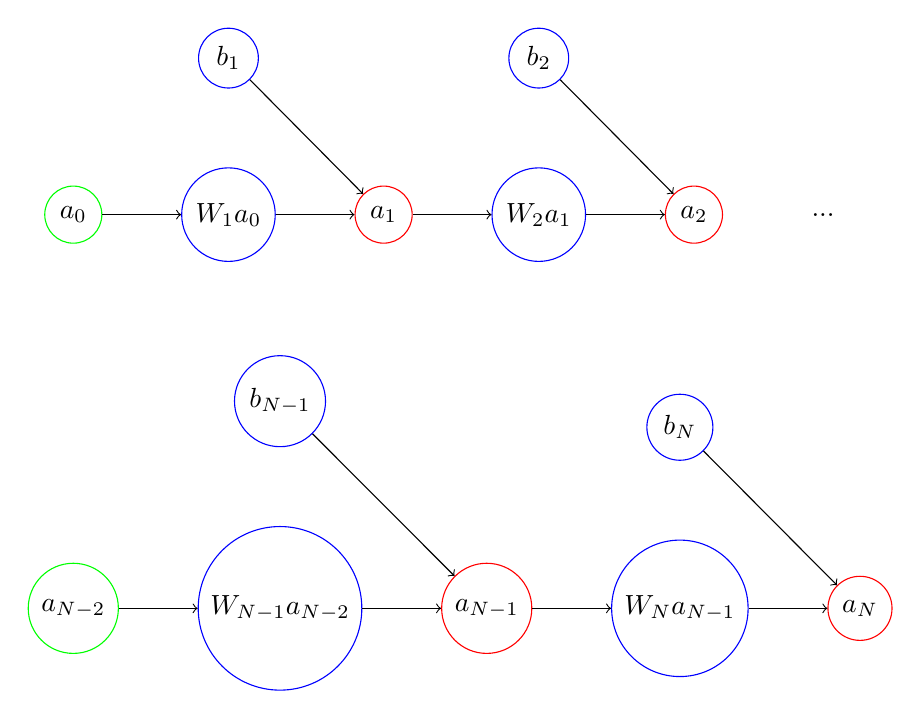
\begin{tikzpicture}[
    inputnode/.style={circle, draw=green},
    outputnode/.style={circle, draw=red},
    comnode/.style={circle, draw=blue},
  ]
  \node[inputnode] (A0)                                {$a_0$};
  \node[comnode]   (W1)        [right= of A0]           {$W_{1}a_{0}$};
  \draw[->] (A0) -- (W1);                         
  \node[comnode]   (B1)        [above= of W1]           {$b_1$};
  \node[outputnode](A1)        [right= of W1]           {$a_1$};
  \draw[->] (W1) -- (A1);                        
  \draw[->] (B1) -- (A1);                         
  \node[comnode]   (W2)        [right= of A1]           {$W_{2}a_{1}$};
  \draw[->] (A1) -- (W2);                         
  \node[comnode]   (B2)        [above= of W2]           {$b_2$};
  \node[outputnode](A2)        [right= of W2]           {$a_2$};
  \draw[->] (W2) -- (A2);                        
  \draw[->] (B2) -- (A2);                         
  \node (dotsnode)             [right=of A2]            {$...$};
  \node[inputnode] (ANm2)      at (0, -5)               {$a_{N-2}$};
  \node[comnode]   (WNm1)      [right= of ANm2]         {$W_{N-1}a_{N-2}$};
  \draw[->] (ANm2) -- (WNm1);                        
  \node[comnode]   (BNm1)      [above= of WNm1]         {$b_{N-1}$};
  \node[outputnode](ANm1)      [right= of WNm1]         {$a_{N-1}$};
  \draw[->] (WNm1) -- (ANm1);                        
  \draw[->] (BNm1) -- (ANm1);                         
  \node[comnode]   (WN)        [right= of ANm1]         {$W_{N}a_{N-1}$};
  \draw[->] (ANm1) -- (WN);                        
  \node[comnode]   (BN)        [above= of WN]           {$b_{N}$};
  \node[outputnode](AN)        [right= of WN]           {$a_{N}$};
  \draw[->] (WN) -- (AN);
  \draw[->] (BN) -- (AN);
\end{tikzpicture}

and denote the cost function

\begin{equation}
  C(W) = \sum_{c=1}^C(a_{N, c} - y_c)^2
\end{equation}

The goal is to find the parameters of the network \(W_1, W_2, .. W_n\) that minimize the cost function.

\begin{align}
  \frac{\partial C}{\partial W_1} = \sum_{c=1}^N 2
\end{align}
\section{Complete network}
\label{sec:org1d9b4ad}
\subsection{Activation function of one layer}
\label{sec:orge7474c6}
\begin{equation}
a_{n}^{k} = \sigma(\sum_{l=1}^{N(k-1)} w_{n, l}^{k} a_{l}^{k-1} + b_{n})
\end{equation}
\subsection{Cost function}
\label{sec:org77fe2e2}
Let:
\begin{itemize}
\item \(T\): the number of trials,
\item \(K\): the number of layers of the network,
\item \(N(k)\): the number of nodes in the \(k\) layer of the network,
\end{itemize}

\begin{equation}
C = \sum_{i=1}^{T}\sum_{n=1}^{N(K)} (a_{n}^{N(K)} - y_{n})^{2}
\end{equation}
\subsubsection{Layer K: Last layer}
\label{sec:org8fe5eb8}
let's try finding the derivatives with the weights of the last layer, \(K\) and lets denote the error of the \(n_{\text{th}}\) output with:

\(\newline\)
\(\epsilon_{n} = (a_{n}^{K} - y_{n})\)

\begin{align}
\frac{\partial C}{\partial w_{c,p}^{K}} &= \sum_{i=1}^{T}\sum_{n=1}^{N(K)} 2\epsilon_{n}\frac{\partial a_{n}^{K}}{\partial w_{c,p}^{K}}
\\
\frac{\partial C}{\partial w_{c,p}^{K}} &= \sum_{i=1}^{T}\sum_{n=1}^{N(K)} 2\epsilon_{n}\frac{\partial \sigma(\sum_{l=1}^{N(K-1)} w_{n, l}^{K} a_{l}^{K-1} + b_{n})}{\partial w_{c,p}^{K}}
\\
\frac{d \sigma(x)}{dx} &= \sigma(x)(1 - \sigma(x))
\\
z_{n}^{K} &= \sum_{l=1}^{N(K-1)} w_{n, l}^{K} a_{l}^{K-1} + b_{n}
\\
\frac{\partial C}{\partial w_{c,p}^{K}} &= \sum_{i=1}^{T}\sum_{n=1}^{N(K)} 2\epsilon_{n}a_{n}^{K}(1-a_{n}^{K})\frac{\partial z_{n}^{K}}{\partial w_{c,p}^{K}}
\\
\frac{\partial C}{\partial w_{c,p}^{K}} &= \sum_{i=1}^{T}2\epsilon_{c}a_{c}^{K}(1-a_{c}^{K})a_{p}^{K-1}
\end{align}

We've found the the derivatives for the weights of the last layer are:
\(\newline\)
\begin{equation}
\frac{\partial C}{\partial w_{c,p}^{K}} = \sum_{i=1}^{T}2\epsilon_{c}a_{c}^{K}(1-a_{c}^{K})a_{p}^{K-1}
\end{equation}
\(\newline\)
Let's define \(2\epsilon_{c}a_{c}^{K}(1-a_{c}^{K})\), the back propagation of the error in \(c\) node of the last layer as \(e_{c}^{K}\).
Then:
\(\newline\)
\begin{equation}
\frac{\partial C}{\partial w_{c,p}^{K}} = \sum_{i=1}^{T}e_{c} a_{p}
\end{equation}
\subsubsection{Layer K - 1}
\label{sec:orgc0c00af}
let's try now with the derivatives of the layer before the last, \(K-1\): 
\begin{align}
\frac{\partial C}{\partial w_{c,p}^{K-1}} &= \sum_{i=1}^{T}\sum_{n=1}^{N(K)} 2\epsilon_{n}\frac{\partial a_{n}^{K}}{\partial w_{c,p}^{K-1}}
\\
\frac{\partial C}{\partial w_{c,p}^{K-1}} &= \sum_{i=1}^{T}\sum_{n=1}^{N(K)} 2\epsilon_{n}\frac{\partial \sigma(\sum_{l=1}^{N(K-1)} w_{n, l}^{K} a_{l}^{K-1} + b_{n})}{\partial w_{c,p}^{K-1}}
\\
z_{n}^{K} &= \sum_{l=1}^{N(K-1)} w_{n, l}^{K} a_{l}^{K-1} + b_{n}
\\
\frac{\partial C}{\partial w_{c,p}^{K-1}} &= \sum_{i=1}^{T}\sum_{n=1}^{N(K)} 2\epsilon_{n}a_{n}^{K}(1-a_{n}^{K})\frac{\partial z_{n}^{K}}{\partial w_{c,p}^{K-1}}
\\
\frac{\partial z_{n}^{K}}{\partial w_{c,p}^{K-1}} &= \frac{\partial \sum_{l=1}^{N(K-1)} w_{n, l}^{K} a_{l}^{K-1} + b_{n}}{\partial w_{c,p}^{K-1}} = \sum_{l=1}^{N(K-1)} w_{n, l}^{K}\frac{\partial a_{l}^{K-1}}{\partial w_{c,p}^{K-1}}
\\
z_{l}^{K-1} &= \sum_{m=1}^{N(K-2)} w_{l, m}^{K-1} a_{m}^{K-2} + b_{l}
\\
\frac{\partial z_{n}^{K}}{\partial w_{c,p}^{K-1}} &= \sum_{l=1}^{N(K-1)} w_{n, l}^{K}a_{l}^{K-1}(1-a_{l}^{K-1})\frac{\partial z_{l}^{K-1}}{\partial w_{c,p}^{K-1}}
\\
\frac{\partial z_{n}^{K-1}}{\partial w_{c,p}^{K-1}} &= a_{p}^{K-2}
\\
\frac{\partial z_{n}^{K}}{\partial w_{c,p}^{K-1}} &= w_{n, c}^{K}a_{c}^{K-1}(1-a_{c}^{K-1})a_{p}^{K-2}
\\
\frac{\partial C}{\partial w_{c,p}^{K-1}} &= \sum_{i=1}^{T}\sum_{n=1}^{N(K)} 2\epsilon_{n}a_{n}^{K}(1-a_{n}^{K})w_{n, c}^{K}a_{c}^{K-1}(1-a_{c}^{K-1})a_{p}^{K-2}
\end{align}


We've found the the derivatives for the weights of layer before the last layer are:
\begin{equation}
\frac{\partial C}{\partial w_{c,p}^{K-1}} = \sum_{i=1}^{T}\sum_{n=1}^{N(K)} 2\epsilon_{n}a_{n}^{K}(1-a_{n}^{K})w_{n, c}^{K}a_{c}^{K-1}(1-a_{c}^{K-1})a_{p}^{K-2}
\end{equation}

You can recognize in the equation the term \(2e_{n}a_{n}^{K}(1-a_{n}^{K})\) to be what we first had defined as the propagation of the error in the \(K\) layer, \(e_{n}^{K}\).

\begin{equation}
\frac{\partial C}{\partial w_{c,p}^{K-1}} = \sum_{i=1}^{T}\sum_{n=1}^{N(K)}e_{n}^{K}w_{n, c}a_{c}^{K-1}(1-a_{c}^{K-1})a_{p}^{K-2}
\end{equation}

and define
\begin{equation}
e_{c}^{K-1} = \sum_{i=1}^{T}\sum_{n=1}^{N(K)}e_{n}^{K}w_{n, c}a_{c}^{K-1}(1-a_{c}^{K-1})
\end{equation}

so that:
\begin{equation}
\frac{\partial C}{\partial w_{c,p}^{K-1}} = \sum_{i=1}^{T}e_c^{K-1}a_{p}^{K-2}
\end{equation}
\subsubsection{Layer K-2}
\label{sec:orgdc136db}
let's try now with the derivatives of two layers before the last, \(K-2\):
\begin{align}
\frac{\partial C}{\partial w_{c,p}^{K-2}} &= \sum_{i=1}^{T}\sum_{n=1}^{N(K)} 2\epsilon_{n}\frac{\partial a_{n}^{K}}{\partial w_{c,p}^{K-2}}
\\
\frac{\partial C}{\partial w_{c,p}^{K-2}} &= \sum_{i=1}^{T}\sum_{n=1}^{N(K)} 2\epsilon_{n}\frac{\partial \sigma(\sum_{l=1}^{N(K-1)} w_{n, l}^{K} a_{l}^{K-1} + b_{n})}{\partial w_{c,p}^{K-2}}
\\
\frac{\partial C}{\partial w_{c,p}^{K-2}} &= \sum_{i=1}^{T}\sum_{n=1}^{N(K)} 2\epsilon_{n}a_{n}^{K}(1-a_{n}^{K})\frac{\partial (\sum_{l=1}^{N(K-1)} w_{n, l}^{K} a_{l}^{K-1} + b_{n})}{\partial w_{c,p}^{K-2}}
\\
\frac{\partial C}{\partial w_{c,p}^{K-2}} &= \sum_{i=1}^{T}\sum_{n=1}^{N(K)} 2\epsilon_{n}a_{n}^{K}(1-a_{n}^{K})(\sum_{l=1}^{N(K-1)} w_{n, l}^{K} \frac{\partial a_{l}^{K-1}}{\partial w_{c,p}^{K-2}})
\\
\frac{\partial C}{\partial w_{c,p}^{K-2}} &= \sum_{i=1}^{T}\sum_{n=1}^{N(K)} 2\epsilon_{n}a_{n}^{K}(1-a_{n}^{K})(\sum_{l=1}^{N(K-1)} w_{n, l}^{K}a_{l}^{K-1}(1-a_{l}^{K-1})\frac{\partial \sum_{m=1}^{N(K-2)} w_{l,m}^{K-1}a_{m}^{K-2} + b_{m}^{K-1}}{\partial w_{c,p}^{K-2}})
\\
\frac{\partial C}{\partial w_{c,p}^{K-2}} &= \sum_{i=1}^{T}\sum_{n=1}^{N(K)} 2\epsilon_{n}a_{n}^{K}(1-a_{n}^{K})(\sum_{l=1}^{N(K-1)} w_{n, l}^{K}a_{l}^{K-1}(1-a_{l}^{K-1})\sum_{m=1}^{N(K-2)} w_{l,m}^{K-1}\frac{\partial a_{m}^{K-2}}{\partial w_{c,p}^{K-2}})
\\
\begin{split}
\frac{\partial C}{\partial w_{c,p}^{K-2}} &= \sum_{i=1}^{T}\sum_{n=1}^{N(K)} 2\epsilon_{n}a_{n}^{K}(1-a_{n}^{K}) \sum_{l=1}^{N(K-1)} w_{n, l}^{K}a_{l}^{K-1}(1-a_{l}^{K-1})\sum_{m=1}^{N(K-2)} w_{l,m}^{K-1}a_{m}^{K-2}(1-a_{m}^{K-2}) \\ &\frac{\partial \sum_{o=1}^{N(K-3)} w_{m,o}^{K-2} a_{o}^{K-3} + b_{m}^{K-2}}{\partial w_{c,p}^{K-2}}
\end{split}
\\
\frac{\partial C}{\partial w_{c,p}^{K-2}} &= \sum_{i=1}^{T}\sum_{n=1}^{N(K)} 2\epsilon_{n}a_{n}^{K}(1-a_{n}^{K})\sum_{l=1}^{N(K-1)} w_{n, l}^{K}a_{l}^{K-1}(1-a_{l}^{K-1})w_{l,c}^{K-1}a_{c}^{K-2}(1-a_{c}^{K-2})a_{p}^{K-3}
\end{align}

So the derivative of the layer \(K-2\) is:

\begin{equation}
\frac{\partial C}{\partial w_{c,p}^{K-2}} = \sum_{i=1}^{T}\sum_{n=1}^{N(K)} 2\epsilon_{n}a_{n}^{K}(1-a_{n}^{K})\sum_{l=1}^{N(K-1)} w_{n, l}^{K}a_{l}^{K-1}(1-a_{l}^{K-1})w_{l,c}^{K-1}a_{c}^{K-2}(1-a_{c}^{K-2})a_{p}^{K-3}
\end{equation}

switching the summatories with \(n\) and \(l\):
\begin{equation}
\frac{\partial C}{\partial w_{c,p}^{K-2}} = \sum_{i=1}^{T}\sum_{l=1}^{N(K-1)}\sum_{n=1}^{N(K)} 2\epsilon_{n}a_{n}^{K}(1-a_{n}^{K})w_{n, l}^{K}a_{l}^{K-1}(1-a_{l}^{K-1})w_{l,c}^{K-1}a_{c}^{K-2}(1-a_{c}^{K-2})a_{p}^{K-3}
\end{equation}

you can see that the term

\begin{equation}
\sum_{n=1}^{N(K)} 2\epsilon_{n}a_{n}^{K}(1-a_{n}^{K})w_{n, l}^{K}a_{l}^{K-1}(1-a_{l}^{K-1})
\end{equation}

is the propagation of the error to the \(l\) element of the \(K-1\) layer, \(e_{l}^{K-1}\). Then you can write:

\begin{equation}
\frac{\partial C}{\partial w_{c,p}^{K-2}} = \sum_{i=1}^{T}\sum_{l=1}^{N(K-1)}e_{l}^{K-1}w_{l,c}^{K-1}a_{c}^{K-2}(1-a_{c}^{K-2})a_{p}^{K-3}
\end{equation}

and denote

\begin{equation}
e_{c}^{K-2} = \sum_{l=1}^{N(K-1)}e_{l}^{K-1}w_{l,c}^{K-1}a_{c}^{K-2}(1-a_{c}^{K-2})
\end{equation}

as the propagation of the error to the \(c\) node of the \(K-2\) layer so that:

\begin{equation}
\frac{\partial C}{\partial w_{c,p}^{K-2}} = e_{c}^{K-2}a_{p}^{K-3}
\end{equation}
\subsection{Generic activation function}
\label{sec:orgd0c2550}

\begin{align}
&z_{i}^{k} = \sum_{j=1}^{N(k-1)} w_{i,j}^{k}a_{j}^{k-1} + b_{i}^{k}
\\
&a_{i}^{k} = \alpha(z_{i}^{k})
\end{align}

\begin{align}
C &= \sum_{t=1}^{T} \sum_{i=1}^{N(K)}(a_{i} - y_{i. t})^{2}
\\
\frac{\partial C}{\partial w_{c, p}^{K}} &= \frac{\partial\sum_{t=1}^{T} \sum_{i=1}^{N(K)}(a_{i}^{K} - y_{i. t})^{2}}{\partial w_{c, p}^{K}}
\\
\frac{\partial C}{\partial w_{c, p}^{K}} &= \sum_{t=1}^{T} \frac{\partial \sum_{i=1}^{N(K)}(a_{i}^{K} - y_{i. t})^{2}}{\partial w_{c, p}^{K}}
\\
\frac{\partial C}{\partial w_{c, p}^{K}} &= \sum_{t=1}^{T} \sum_{i=1}^{N(K)} \frac{\partial (a_{i}^{K} - y_{i. t})^{2}}{\partial w_{c, p}^{K}}
\\
\frac{\partial C}{\partial w_{c, p}^{K}} &= \sum_{t=1}^{T} \sum_{i=1}^{N(K)} 2(a_{i}^{K} - y_{i. t}) \frac{d a_{i}^{K}}{d z_{i}^{K}}\frac{\partial z_{i}^{K}}{\partial w_{c, p}^{K}}
\\
\frac{\partial z_{i}^{K}}{\partial w_{c, p}^{K}} &= \frac{\partial \sum_{j=1}^{L(n-1)} w_{j,i}^{n}a_{j}^{n-1} + b_{i}^{n}}{\partial w_{c, p}^{K}}
\\
\frac{\partial z_{i}^{K}}{\partial w_{c, p}^{K}} &= \sum_{j=1}^{N(K-1)} \frac{\partial w_{i,j}^{K}a_{j}^{K-1} + b_{i}^{K}}{\partial w_{c, p}^{K}}
\\
\frac{\partial C}{\partial w_{c, p}^{K}} &= \sum_{t=1}^{T} \sum_{i=1}^{N(K)} 2(a_{i}^{K} - y_{i. t}) \frac{d a_{i}^{K}}{d z_{i}^{K}}\sum_{j=1}^{N(K-1)} \frac{\partial (w_{i,j}^{K}a_{j}^{K-1} + b_{i}^{K})}{\partial w_{c, p}^{K}}
\\
\frac{\partial C}{\partial w_{c, p}^{K}} &= \sum_{t=1}^{T} 2(a_{c}^{K} - y_{c, t}) \frac{d a_{c}^{K}}{d z_{c}^{K}}a_{p}^{K-1}
\end{align}


\begin{align}
\frac{\partial C}{\partial w_{c, p}^{K-1}} &= \frac{\partial\sum_{t=1}^{T} \sum_{i=1}^{N(K)}(a_{i}^{K} - y_{i. t})^{2}}{\partial w_{c, p}^{K}}
\\
\frac{\partial C}{\partial w_{c, p}^{K-1}} &= \sum_{t=1}^{T} \sum_{i=1}^{N(K)} 2(a_{i}^{K} - y_{i. t}) \frac{d a_{i}^{K}}{d z_{i}^{K}}\sum_{j=1}^{N(K-1)} \frac{\partial (w_{i,j}^{K}a_{j}^{K-1} + b_{i}^{K})}{\partial w_{c, p}^{K-1}}
\\
\frac{\partial C}{\partial w_{c, p}^{K-1}} &= \sum_{t=1}^{T} \sum_{i=1}^{N(K)} 2(a_{i}^{K} - y_{i. t}) \frac{d a_{i}^{K}}{d z_{i}^{K}}\sum_{j=1}^{N(K-1)} \frac{\partial (w_{i,j}^{K}a_{j}^{K-1} + b_{i}^{K})}{\partial w_{c, p}^{K-1}}
\\
\frac{\partial C}{\partial w_{c, p}^{K-1}} &= \sum_{t=1}^{T} \sum_{i=1}^{N(K)} 2(a_{i}^{K} - y_{i. t}) \frac{d a_{i}^{K}}{d z_{i}^{K}}\sum_{j=1}^{N(K-1)} w_{i,j}^{K} \frac{\partial a_{j}^{K-1}}{\partial w_{c, p}^{K-1}}
\\
\frac{\partial C}{\partial w_{c, p}^{K-1}} &= \sum_{t=1}^{T} \sum_{i=1}^{N(K)} 2(a_{i}^{K} - y_{i. t}) \frac{d a_{i}^{K}}{d z_{i}^{K}}\sum_{j=1}^{N(K-1)} w_{i,j}^{K} \frac {d a_{j}^{K-1}}{d z_{j}^{K-1}} \frac{\partial z_{j}^{K-1}}{\partial w_{c, p}^{K-1}}
\\
\frac{\partial z_{j}^{K-1}}{\partial w_{c, p}^{K-1}} &= \frac{\partial \sum_{n=1}^{N(K-2)} w_{j,n}^{K-1}a_{n}^{K-2} + b_{j}^{K-1}}{\partial w_{c, p}^{K-1}}
\\
\frac{\partial z_{j}^{K-1}}{\partial w_{c, p}^{K-1}} &= \sum_{n=1}^{N(K-2)} \frac{\partial (w_{j,n}^{K-1}a_{n}^{K-2} + b_{j}^{K-1})}{\partial w_{c, p}^{K-1}}
\\
\frac{\partial C}{\partial w_{c, p}^{K-1}} &= \sum_{t=1}^{T} \sum_{i=1}^{N(K)} 2(a_{i}^{K} - y_{i. t}) \frac{d a_{i}^{K}}{d z_{i}^{K}}\sum_{j=1}^{N(K-1)} w_{i,j}^{K} \frac {d a_{j}^{K-1}}{d z_{j}^{K-1}}\sum_{n=1}^{N(K-2)} \frac{\partial (w_{j,n}^{K-1}a_{n}^{K-2} + b_{j}^{K-1})}{\partial w_{c, p}^{K-1}}
\\
\frac{\partial C}{\partial w_{c, p}^{K-1}} &= \sum_{t=1}^{T} \sum_{i=1}^{N(K)} 2(a_{i}^{K} - y_{i. t}) \frac{d a_{i}^{K}}{d z_{i}^{K}}w_{i,c}^{K} \frac {d a_{c}^{K-1}}{d z_{c}^{K-1}} a_{p}^{K-2}
\end{align}
\end{document}
